% Copyright 2004 by Till Tantau <tantau@users.sourceforge.net>.
%
% In principle, this file can be redistributed and/or modified under
% the terms of the GNU Public License, version 2.
%
% However, this file is supposed to be a template to be modified
% for your own needs. For this reason, if you use this file as a
% template and not specifically distribute it as part of a another
% package/program, I grant the extra permission to freely copy and
% modify this file as you see fit and even to delete this copyright
% notice. 

\documentclass{beamer}

\usepackage{graphicx}
\usepackage{pgf}
\usepackage{tikz}
\usepackage{listings}
\lstset{
    language=HTML,
    tabsize=8,
    keepspaces,
    extendedchars=true,
    rulecolor=\color{black},
    basicstyle=\footnotesize,
    aboveskip=5pt,
    upquote=true,
    columns=fixed,
    showstringspaces=false,
    extendedchars=true,
    breaklines=true,
    frame=single,
    showtabs=true,
    showspaces=false,
    showstringspaces=false,
}
\usetikzlibrary{arrows,automata,positioning}

\beamertemplatenavigationsymbolsempty

% There are many different themes available for Beamer. A comprehensive
% list with examples is given here:
% http://deic.uab.es/~iblanes/beamer_gallery/index_by_theme.html
% You can uncomment the themes below if you would like to use a different
% one:
%\usetheme{AnnArbor}
%\usetheme{Antibes}
%\usetheme{Bergen}
%\usetheme{Berkeley}
%\usetheme{Berlin}
%\usetheme{Boadilla}
%\usetheme{boxes}
%\usetheme{CambridgeUS}
%\usetheme{Copenhagen}
%\usetheme{Darmstadt}
%\usetheme{default}
%\usetheme{Frankfurt}
%\usetheme{Goettingen}
%\usetheme{Hannover}
%\usetheme{Ilmenau}
%\usetheme{JuanLesPins}
%\usetheme{Luebeck}
\usetheme{Madrid}
%\usetheme{Malmoe}
%\usetheme{Marburg}
%\usetheme{Montpellier}
%\usetheme{PaloAlto}
%\usetheme{Pittsburgh}
%\usetheme{Rochester}
%\usetheme{Singapore}
%\usetheme{Szeged}
%\usetheme{Warsaw}

\title{Introduction to Ranked Tree Automata}


\author{Martin Braun}
% - Give the names in the same order as the appear in the paper.
% - Use the \inst{?} command only if the authors have different
%   affiliation.

\institute[University of Bayreuth] % (optional, but mostly needed)
{
	University of Bayreuth
}
% - Use the \inst command only if there are several affiliations.
% - Keep it simple, no one is interested in your street address.

\date{30.04.2014}
% - Either use conference name or its abbreviation.
% - Not really informative to the audience, more for people (including
%   yourself) who are reading the slides online

\subject{Theoretical Computer Science}
% This is only inserted into the PDF information catalog. Can be left
% out. 

% If you have a file called "university-logo-filename.xxx", where xxx
% is a graphic format that can be processed by latex or pdflatex,
% resp., then you can add a logo as follows:

% \pgfdeclareimage[height=0.5cm]{university-logo}{university-logo-filename}
% \logo{\pgfuseimage{university-logo}}

% Delete this, if you do not want the table of contents to pop up at
% the beginning of each subsection:
%\AtBeginSubsection[]
%{
%  \begin{frame}<beamer>{Outline}
%    \tableofcontents[currentsection,currentsubsection]
%  \end{frame}
%}

% Let's get started
\begin{document}

\begin{frame}
  \titlepage
   \begin{center}
	Supervisor: Prof. Dr. Wim Martens
   \end{center}
\end{frame}

\newcommand{\nfaExample}{
	 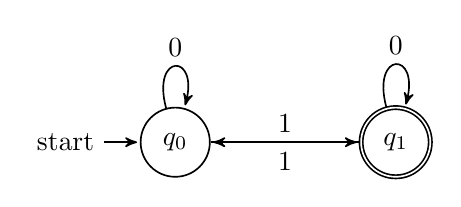
\begin{tikzpicture}[->,>=stealth',shorten >=1pt,auto,node distance=2.8cm,
                 		   semithick]
 				\tikzstyle{every state}=[fill=white,draw=black,text=black]
		
				\node[initial,state]		(A)			{$q_0$};
				\node[state,accepting]	(B)	[right of=A]	{$q_1$};
	
 				 \path (A)	edge	[loop above]	node {0}	(A)
					(A)	edge			node {1}	(B)
					(B)	edge	[loop above]	node {0}	(B)
					(B)	edge			node {1}	(A);
	\end{tikzpicture}
}

\newcommand{\nfaExampleActiveInitial}{
 	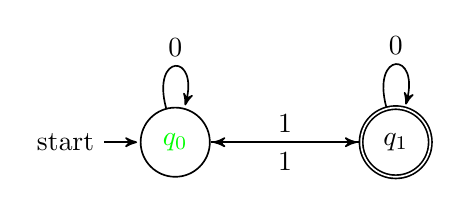
\begin{tikzpicture}[->,>=stealth',shorten >=1pt,auto,node distance=2.8cm,
                 		   semithick]
 				\tikzstyle{every state}=[fill=white,draw=black,text=black]
		
				\node[initial,state]		(A)			{\textcolor{green}{$q_0$}};
				\node[state,accepting]	(B)	[right of=A]	{$q_1$};
	
 				 \path (A)	edge	[loop above]	node {0}	(A)
					(A)	edge			node {1}	(B)
					(B)	edge	[loop above]	node {0}	(B)
					(B)	edge			node {1}	(A);
	\end{tikzpicture}
}

\newcommand{\nfaExampleActiveFinal}{
 	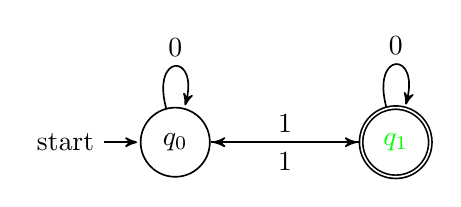
\begin{tikzpicture}[->,>=stealth',shorten >=1pt,auto,node distance=2.8cm,
                 		   semithick]
 				\tikzstyle{every state}=[fill=white,draw=black,text=black]
		
				\node[initial,state]		(A)			{$q_0$};
				\node[state,accepting]	(B)	[right of=A]	{\textcolor{green}{$q_1$}};
	
 				 \path (A)	edge	[loop above]	node {0}	(A)
					(A)	edge			node {1}	(B)
					(B)	edge	[loop above]	node {0}	(B)
					(B)	edge			node {1}	(A);
	\end{tikzpicture}
}

\begin{frame}{A first example}{A look back to NFAs/DFAs}
	\begin{center}
    			\nfaExample
	\end{center}
	\pause
	\begin{center}
		This DFA accepts all \textcolor{green}{strings} with an odd number of 1's
	\end{center}
	\pause
	\begin{block}{}
		NFAs/DFAs consist of:
		\begin{itemize}
			\item {
				a finite set of states \(Q\)
			}
			\item {
				a finite set of input symbols \(\Sigma\)
			}
			\item {
				a transitional relation \(\Delta : Q \times \Sigma \rightarrow Q\) 
			}
			\item {
				an initial state \(q_0 \in Q\)
			}
			\item {
				a set of final states \(Q_f \subseteq Q\)
			}
		\end{itemize}
		\pause
		They are used to recognize \textcolor{green}{strings}.
	\end{block}
\end{frame}

\newcommand{\simpleTreeExample} {
	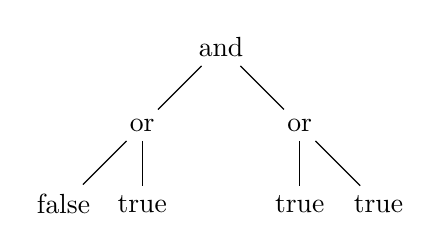
\begin{tikzpicture}[auto]
			\node (and) at (2, 3) {and};
			\node (or1) at (1, 2) {or};
			\node (or2) at (3, 2) {or};
			\node (false1) at (0, 1) {false};
			\node (true1) at (1, 1) {true};
			\node (true2) at (3, 1) {true};
			\node (true3) at (4, 1) {true};

			\draw [-] (and) to (or1);
			\draw [-] (and) to (or2);
			\draw [-] (or1) to (false1);
			\draw [-] (or1) to (true1);
			\draw [-] (or2) to (true2);
			\draw [-] (or2) to (true3);
	\end{tikzpicture}
}

\begin{frame}{A first example}{Strings are nice, but...}
	\begin{block}{}
		...what about languages that have an inherent structure?
	\end{block}
	\pause
	\begin{center}
		\simpleTreeExample
		\:\:
		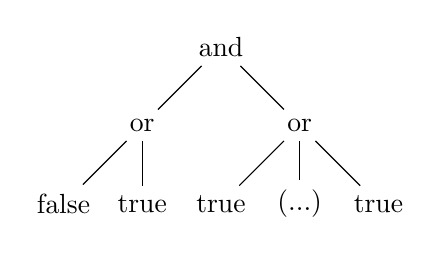
\begin{tikzpicture}[auto]
			\node (and) at (2, 3) {and};
			\node (or1) at (1, 2) {or};
			\node (or2) at (3, 2) {or};
			\node (false1) at (0, 1) {false};
			\node (true1) at (1, 1) {true};
			\node (true2) at (2, 1) {true};
			\node (rest) at (3, 1) {(...)};
			\node (true3) at (4, 1) {true};

			\draw [-] (and) to (or1);
			\draw [-] (and) to (or2);
			\draw [-] (or1) to (false1);
			\draw [-] (or1) to (true1);
			\draw [-] (or2) to (true2);
			\draw [-] (or2) to (rest);
			\draw [-] (or2) to (true3);
		\end{tikzpicture}
	\end{center}
	\pause
	\begin{center}
		What if we want to recognize a \textcolor{green}{tree-language} that consists of all true boolean statements?
	\end{center}
\end{frame}

\begin{frame}{A first example}{}
	\begin{center}
		\nfaExample
		\begin{block}{}
			 Now consider a \textcolor{green}{run} on this NFA with the input:
			\newline
			0 1 1 1
		\end{block}
		\begin{tikzpicture}[auto]
			\node (node3) at (0, 3) {1};
			\node (node2) at (0, 2) {1};
			\node (node1) at (0, 1) {1};
			\node (node0) at (0, 0) {0};

			\draw [-] (node3) to (node2);
			\draw [-] (node2) to (node1);
			\draw [-] (node1) to (node0);
		\end{tikzpicture}
	\end{center}
\end{frame}

\begin{frame}{A first example}{}
	\begin{center}
		\nfaExampleActiveInitial
		\begin{block}{}
				Input:
				\newline
				\textcolor{green}{0} 1 1 1
			\end{block}
		\begin{tikzpicture}[auto]
				\node (node3) at (0, 3) {1};
				\node (node2) at (0, 2) {1};
				\node (node1) at (0, 1) {1};
				\node (node0) at (0, 0) {0};
				\node at (2, 0) {\textcolor{green}{\( 0(q_0) \rightarrow q_0 \)}};
	
				\draw [-] (node3) to (node2);
				\draw [-] (node2) to (node1);
				\draw [-] (node1) to (node0);
		\end{tikzpicture}
	\end{center}
\end{frame}

\begin{frame}{A first example}{}
	\begin{center}
	\nfaExampleActiveFinal
	\begin{block}{}
			Input:
			\newline
			\textcolor{red}{0} \textcolor{green}{1} 1 1
		\end{block}
	\begin{tikzpicture}[auto]
			\node (node3) at (0, 3) {1};
			\node (node2) at (0, 2) {1};
			\node (node1) at (0, 1) {1};
			\node at (2, 1) {\textcolor{green}{\( 1(q_0) \rightarrow q_1 \)}};
			\node (node0) at (0, 0) {0};
			\node at (2, 0) {$q_0$};

			\draw [-] (node3) to (node2);
			\draw [-] (node2) to (node1);
			\draw [-] (node1) to (node0);
	\end{tikzpicture}
	\end{center}
\end{frame}

\begin{frame}{A first example}{}
	\begin{center}
	\nfaExampleActiveInitial
	\begin{block}{}
			Input:
			\newline
			\textcolor{red}{0 1} \textcolor{green}{1} 1
		\end{block}
	\begin{tikzpicture}[auto]
			\node (node3) at (0, 3) {1};
			\node (node2) at (0, 2) {1};
			\node at (2, 2) {\textcolor{green}{\( 1(q_1) \rightarrow q_0 \)}};
			\node (node1) at (0, 1) {1};
			\node at (2, 1) {$q_1$};
			\node (node0) at (0, 0) {0};
			\node at (2, 0) {$q_0$};

			\draw [-] (node3) to (node2);
			\draw [-] (node2) to (node1);
			\draw [-] (node1) to (node0);
	\end{tikzpicture}
	\end{center}
\end{frame}

\begin{frame}{A first example}{}
	\begin{center}
	\nfaExampleActiveFinal
	\begin{block}{}
			Input:
			\newline
			\textcolor{red}{0 1 1} \textcolor{green}{1}
		\end{block}
	\begin{tikzpicture}[auto]
			\node (node3) at (0, 3) {1};
			\node at (2, 3) {\textcolor{green}{\( 1(q_0) \rightarrow q_1 \)}};
			\node (node2) at (0, 2) {1};
			\node at (2, 2)  {$q_0$};
			\node (node1) at (0, 1) {1};
			\node at (2, 1) {$q_1$};
			\node (node0) at (0, 0) {0};
			\node at (2, 0) {$q_0$};

			\draw [-] (node3) to (node2);
			\draw [-] (node2) to (node1);
			\draw [-] (node1) to (node0);
	\end{tikzpicture}
	\end{center}
\end{frame}

\begin{frame}{A first example}{}
	\begin{center}
	\nfaExampleActiveFinal
	\begin{block}{}
			Input:
			\newline
			\textcolor{red}{0 1 1 1}. Finished.
			\newline
			\(State(nfa) = q_1 \implies Input \in L(nfa)\)
	\end{block}
	\begin{tikzpicture}[auto]
			\node (node3) at (0, 3) {1};
			\node at (2, 3) {$q_1$};
			\node (node2) at (0, 2) {1};
			\node at (2, 2)  {$q_0$};
			\node (node1) at (0, 1) {1};
			\node at (2, 1) {$q_1$};
			\node (node0) at (0, 0) {0};
			\node at (2, 0) {$q_0$};

			\draw [-] (node3) to (node2);
			\draw [-] (node2) to (node1);
			\draw [-] (node1) to (node0);
	\end{tikzpicture}
	\end{center}
\end{frame}

\begin{frame}{From NFA to NFTA}{BinaryCounter (1)}
	\begin{example}
		We expand our NFA to count the 1's and 0's in "parallel".
		Normal strings aren't sufficient. A restructuration of the input is needed.
	\end{example}
	\pause
	\begin{example}
		For 0 1 1 1 :
		\begin{center}
			\begin{tikzpicture}[auto]
				\node (top) at (1, 2) {\(\epsilon\)};
				\node (node3) at (2, 1) {1};
				\node (node2) at (2, 0) {1};
				\node (node1) at (0, 1) {1};
				\node (node0) at (0, 0) {0};
	
				\draw [-] (top) to (node1);
				\draw [-] (top) to (node3);
				\draw [-] (node3) to (node2);
				\draw [-] (node1) to (node0);
			\end{tikzpicture}
		\end{center}
	\end{example}
\end{frame}

\begin{frame}{From NFA to NFTA}{BinaryCounter (2)}
	\begin{center}
		\nfaExample
	\end{center}
	\begin{center}
		\begin{tikzpicture}[auto]
			\node (top) at (1, 2) {\(\epsilon\)};
			\node (node3) at (2, 1) {1};
			\node (node2) at (2, 0) {1};
			\node (node1) at (0, 1) {1};
			\node (node0) at (0, 0) {0};
					
			\draw [-] (top) to (node1);
			\draw [-] (top) to (node3);
			\draw [-] (node3) to (node2);
			\draw [-] (node1) to (node0);
		\end{tikzpicture}
	\end{center}
\end{frame}

\begin{frame}{From NFA to NFTA}{BinaryCounter (3)}
	\begin{center}
		\nfaExample
	\end{center}
	\begin{center}
		\begin{tikzpicture}[auto]
			\node (top) at (1, 2) {\(\epsilon\)};
			\node (node3) at (2, 1) {1};			
			\node (node2) at (2, 0) {\textcolor{green}{$q_1$}};
			\node at (4, 0) {\textcolor{green}{ \(  1(q_0) \rightarrow q_1 \) }};
			\node (node1) at (0, 1) {1};
			\node (node0) at (0, 0) {\textcolor{green}{$q_0$}};
			\node at (-2, 0) {\textcolor{green}{ \(  0(q_0) \rightarrow q_0 \) }};
					
			\draw [-] (top) to (node1);
			\draw [-] (top) to (node3);
			\draw [-] (node3) to (node2);
			\draw [-] (node1) to (node0);
		\end{tikzpicture}
	\end{center}
\end{frame}

\begin{frame}{From NFA to NFTA}{BinaryCounter (4)}
	\begin{center}
		\nfaExample
	\end{center}
	\begin{center}
		\begin{tikzpicture}[auto]
			\node (top) at (1, 2) {\(\epsilon\)};
			\node (node3) at (2, 1) {\textcolor{green}{$q_0$}};	
			\node at (-2, 1) {\textcolor{green}{ \(  1(q_0) \rightarrow q_1 \) }};		
			\node (node2) at (2, 0) {$q_1$};
			\node (node1) at (0, 1) {\textcolor{green}{$q_1$}};
			\node at (4, 1) {\textcolor{green}{ \(  1(q_1) \rightarrow q_0 \) }};
			\node (node0) at (0, 0) {$q_0$};
					
			\draw [-] (top) to (node1);
			\draw [-] (top) to (node3);
			\draw [-] (node3) to (node2);
			\draw [-] (node1) to (node0);
		\end{tikzpicture}
	\end{center}
\end{frame}

\begin{frame}{From NFA to NFTA}{BinaryCounter (5)}
	\begin{center}
		\nfaExample
	\end{center}
	\begin{center}
		\begin{tikzpicture}[auto]
			\node (top) at (1, 2) {\textcolor{green}{$q_1$}};
			\node at (4, 2) {\textcolor{green}{ \(  \epsilon(q_0, q_1) \rightarrow q_1 \) }};
			\node (node3) at (2, 1) {$q_0$};
			\node (node2) at (2, 0) {$q_1$};
			\node (node1) at (0, 1) {$q_1$};
			\node (node0) at (0, 0) {$q_0$};
					
			\draw [-] (top) to (node1);
			\draw [-] (top) to (node3);
			\draw [-] (node3) to (node2);
			\draw [-] (node1) to (node0);
		\end{tikzpicture}
	\end{center}
\end{frame}

\begin{frame}{From NFA to NFTA}{BinaryCounter (6)}
	\begin{center}
		\nfaExample
	\end{center}
	\begin{center}
		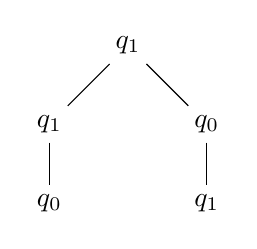
\begin{tikzpicture}[auto]
			\node (top) at (1, 2) {$q_1$};
			\node (node3) at (2, 1) {$q_0$};
			\node (node2) at (2, 0) {$q_1$};
			\node (node1) at (0, 1) {$q_1$};
			\node (node0) at (0, 0) {$q_0$};
					
			\draw [-] (top) to (node1);
			\draw [-] (top) to (node3);
			\draw [-] (node3) to (node2);
			\draw [-] (node1) to (node0);
		\end{tikzpicture}
	\end{center}
	\pause
	\textcolor{green}{Accepted.}
\end{frame}

\begin{frame}{From NFA to NFTA}
	\begin{block}{NFTAs}
		NFTAs behave the same as NFAs except for \(\Delta\).
		They \textcolor{green}{can} have more than one state as a arguments to their terms, i.e.: \(term(q_m, q_n) \rightarrow q_x\)
	\end{block}
\end{frame}

\newcommand{\automatonDefinition} {
 	\(A = (Q, \Sigma, Q_f, \Delta)\)
}

\newcommand{\oneReduction} {
	\(\underset{A}{\rightarrow}\)
}

\newcommand{\multipleReductions} {
	 \(\overset{\ast}{\underset{A}{\rightarrow}}\)
}

\begin{frame}{From NFA to NFTA}{BooleanEvaluator (1)}
	\begin{center}
		\simpleTreeExample
	\end{center}
\end{frame}

\begin{frame}{From NFA to NFTA}{BooleanEvaluator (2)}
	\begin{center}
		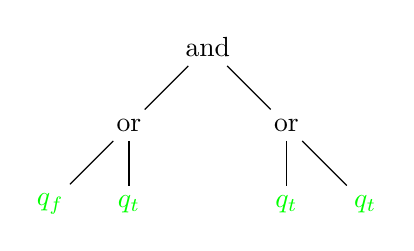
\begin{tikzpicture}[auto]
				\node (and) at (2, 3) {and};
				\node (or1) at (1, 2) {or};
				\node (or2) at (3, 2) {or};
				\node (false1) at (0, 1) {\textcolor{green}{$q_f$}};
				\node (true1) at (1, 1) {\textcolor{green}{$q_t$}};
				\node (true2) at (3, 1) {\textcolor{green}{$q_t$}};
				\node (true3) at (4, 1) {\textcolor{green}{$q_t$}};
						
				\draw [-] (and) to (or1);
				\draw [-] (and) to (or2);
				\draw [-] (or1) to (false1);
				\draw [-] (or1) to (true1);
				\draw [-] (or2) to (true2);
				\draw [-] (or2) to (true3);
		\end{tikzpicture}
	\end{center}	
	\begin{block}{}
		\begin{itemize}
			\item{
				\(false \rightarrow q_f\)
			}
			\item{
				\(true \rightarrow q_t\)
			}
		\end{itemize}
	\end{block}
\end{frame}

\begin{frame}{From NFA to NFTA}{BooleanEvaluator (3)}

	\begin{center}
		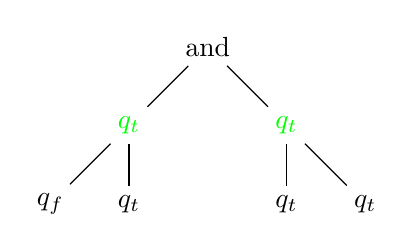
\begin{tikzpicture}[auto]
				\node (and) at (2, 3) {and};
				\node (or1) at (1, 2) {\textcolor{green}{$q_t$}};
				\node (or2) at (3, 2) {\textcolor{green}{$q_t$}};
				\node (false1) at (0, 1) {$q_f$};
				\node (true1) at (1, 1) {$q_t$};
				\node (true2) at (3, 1) {$q_t$};
				\node (true3) at (4, 1) {$q_t$};

				\draw [-] (and) to (or1);
				\draw [-] (and) to (or2);
				\draw [-] (or1) to (false1);
				\draw [-] (or1) to (true1);
				\draw [-] (or2) to (true2);
				\draw [-] (or2) to (true3);
		\end{tikzpicture}
	\end{center}

	\begin{block}{}
		\begin{itemize}
			\item{
				\(or(q_f,q_t) \rightarrow q_t\)
			}
			\item{
				\(or(q_t,q_t) \rightarrow q_t\)
			}
		\end{itemize}
	\end{block}

\end{frame}

\begin{frame}{From NFA to NFTA}{BooleanEvaluator (4)}

	\begin{center}
		\begin{tikzpicture}[auto]
				\node (and) at (2, 3) {\textcolor{green}{$q_t$}};
				\node (or1) at (1, 2) {$q_t$};
				\node (or2) at (3, 2) {$q_t$};
				\node (false1) at (0, 1) {$q_f$};
				\node (true1) at (1, 1) {$q_t$};
				\node (true2) at (3, 1) {$q_t$};
				\node (true3) at (4, 1) {$q_t$};

				\draw [-] (and) to (or1);
				\draw [-] (and) to (or2);
				\draw [-] (or1) to (false1);
				\draw [-] (or1) to (true1);
				\draw [-] (or2) to (true2);
				\draw [-] (or2) to (true3);
		\end{tikzpicture}
	\end{center}

	\begin{block}{}
		\begin{itemize}
			\item{
				\(and(q_t,q_t) \rightarrow q_t\)
			}
		\end{itemize}
	\end{block}

\end{frame}

\begin{frame}{From NFA to NFTA}{BooleanEvaluator (5)}

	\begin{center}
		\begin{tikzpicture}[auto]
				\node (and) at (2, 3) {$q_t$};
				\node (or1) at (1, 2) {$q_t$};
				\node (or2) at (3, 2) {$q_t$};
				\node (false1) at (0, 1) {$q_f$};
				\node (true1) at (1, 1) {$q_t$};
				\node (true2) at (3, 1) {$q_t$};
				\node (true3) at (4, 1) {$q_t$};

				\draw [-] (and) to (or1);
				\draw [-] (and) to (or2);
				\draw [-] (or1) to (false1);
				\draw [-] (or1) to (true1);
				\draw [-] (or2) to (true2);
				\draw [-] (or2) to (true3);
		\end{tikzpicture}
	\end{center}
	\pause
	\textcolor{green}{Accepted.}
	
\end{frame}

\begin{frame}{From NFA to NFTA}{The formal BooleanEvaluator}
	\begin{example}
		Our boolean tree-NFTA is therefore defined as:
		\begin{itemize}
			\item { 
				\automatonDefinition
			}
			\pause
			\item {
				\(\Sigma = \{or, and, not, true,false\}\)
			}
			\pause
			\item {
				\(Q = \{q_f,q_t\}\)
			}
			\pause
			\item {
				\(Q_f = \{q_t\}\)
			}
			\pause
			\item {
				\(\Delta = \{ false \rightarrow q_f, true \rightarrow q_t,
					\newline
					 and(q_t, q_t) \rightarrow q_t, and(q_t, q_f) \rightarrow q_f,...,
					\newline
					or(q_t,q_t) \rightarrow q_t, or(q_t, q_f) \rightarrow q_t,...,
					\newline
					not(q_f) \rightarrow q_t, not(q_t) \rightarrow q_f\}\)
			}
		\end{itemize}
		\pause
		This NFTA regonizes all boolean expressions that evaluate to \textcolor{green}{\(true\)}.
	\end{example}
\end{frame}

\begin{frame}{Some additions...}{...to the definition (1)}
	\begin{definition}
		A tree automaton with no two rules of the type
		\begin{itemize}
			\item{
				\(f(q_1,..., q_n) \rightarrow q_x\)
			}
			\item{
				\(f(q_1,...,q_n) \rightarrow q_y\)
			}
		\end{itemize}
		with \(q_x \neq q_y\) and no rules of the type 
		\begin{itemize}
			\item {
				\(\epsilon(q_1, ..., q_n) \rightarrow q_x\)
			}
		\end{itemize}
		is called \textcolor{green}{deterministic.} (DFTA)
	\end{definition}
\end{frame}

\begin{frame}{Determinization}{What we already know (1)}
	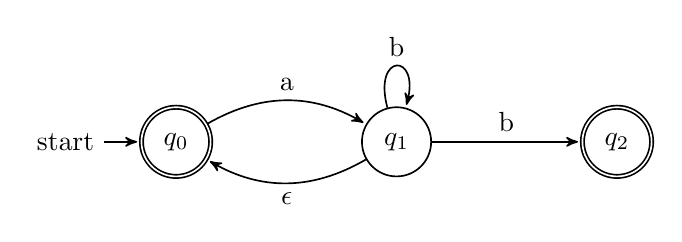
\begin{tikzpicture}[->,>=stealth',shorten >=1pt,auto,node distance=2.8cm,
                 		   semithick]
 				\tikzstyle{every state}=[fill=white,draw=black,text=black]
		
				\node[initial,state, accepting]		(A)			{$q_0$};
				\node[state]					(B)	[right of=A]	{$q_1$};
				\node[state, accepting]			(C)	[right of=B]	{$q_2$};
	
 				 \path (A)	edge	[bend left]		node {a}		(B)
					(B)	edge	[bend left]		node {\(\epsilon\)}	(A)
					(B)	edge	[loop above]		node {b}		(B)
					(B)	edge				node {b}		(C);
	\end{tikzpicture}
	\pause
	\begin{block}{}
		How it's done:
		\begin{itemize}
			\item {
				Use \(\epsilon-closure(q)\) instead of \(q\) for all \(q \in Q\)
			}
			\item {
				Start with the initial state
			}
			\item {
				Generate target states "on the fly" (=set of possible states in original \(Q\))
			}
			\item {
				Repeat for all states including the newly generated ones
			}
		\end{itemize}
	\end{block}
\end{frame}

\begin{frame}{Determinization}{What we already know (2)}
	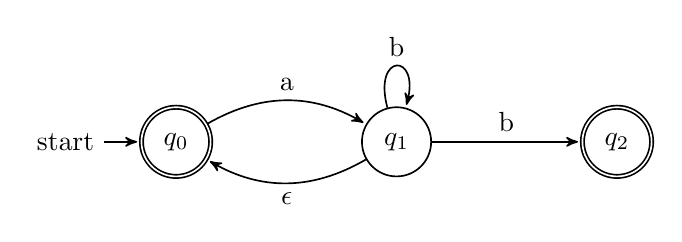
\begin{tikzpicture}[->,>=stealth',shorten >=1pt,auto,node distance=2.8cm,
                 		   semithick]
 				\tikzstyle{every state}=[fill=white,draw=black,text=black]
		
				\node[initial,state, accepting]		(A)			{$q_0$};
				\node[state]					(B)	[right of=A]	{$q_1$};
				\node[state, accepting]			(C)	[right of=B]	{$q_2$};
	
 				 \path (A)	edge	[bend left]		node {a}		(B)
					(B)	edge	[bend left]		node {\(\epsilon\)}	(A)
					(B)	edge	[loop above]		node {b}		(B)
					(B)	edge				node {b}		(C);
	\end{tikzpicture}
	\begin{block}{}
		\begin{itemize}
			\item {
				Initial state: \(\{q_0\}\)
			}
			\pause
			\item {
				\(a(\{q_0\}) \rightarrow \{q_0,q_1\}\) \(\in Q'_f\)
			}
			\pause
			\item {
				\(a(\{q_0,q_1\}) \rightarrow \{q_0,q_1\}\) \newline
				\(b(\{q_0,q_1\}) \rightarrow \{q_0,q_1,q_2\}\) \(\in Q'_f\)
			}
			\pause
			\item {
				\(a(\{q_0,q_1,q_2\}) \rightarrow \{q_0,q_1\}\) \newline
				\(b(\{q_0,q_1,q_2\}) \rightarrow \{q_0,q_1,q_2\}\)
			}
		\end{itemize}
	\end{block}
\end{frame}

\begin{frame}{Determinization}{What we already know (3)}	
	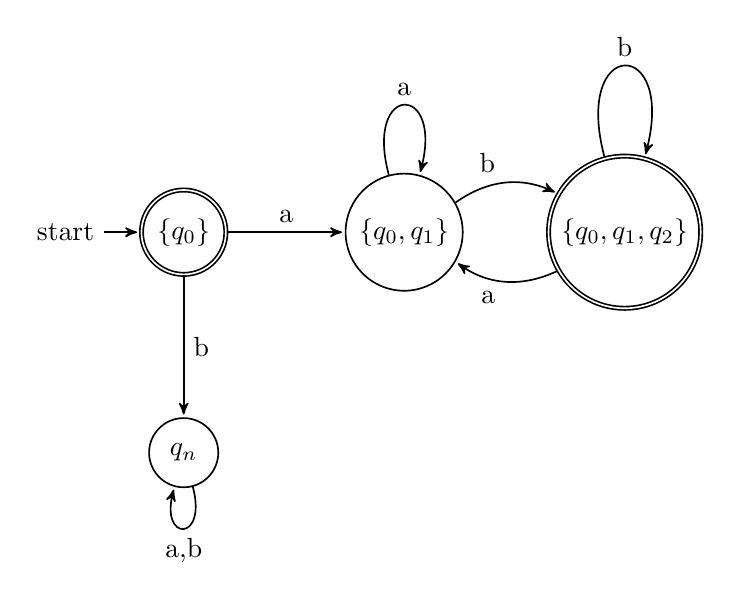
\begin{tikzpicture}[->,>=stealth',shorten >=1pt,auto,node distance=2.8cm,
                 		   semithick]
 				\tikzstyle{every state}=[fill=white,draw=black,text=black]
		
				\node[initial,state, accepting]		(A)			{\(\{q_0\}\)};
				\node[state]					(B)	[right of=A]	{\(\{q_0,q_1\}\)};
				\node[state, accepting]			(C)	[right of=B]	{\(\{q_0,q_1,q_2\}\)};
				\node[state]					(D)	[below of=A] {$q_n$};
	
 				 \path (A)	edge				node {a}		(B)
					(B)	edge	[loop above]		node {a}		(B)
					(B)	edge	[bend left]		node {b}		(C)
					(C)	edge	[bend left]		node {a}		(B)
					(C)	edge	[loop above]		node {b}		(C)
					(A)	edge				node {b}		(D)
					(D)	edge	[loop below]		node {a,b}		(D);
	\end{tikzpicture}
\end{frame}

\begin{frame}{Determinization}{Now for NFTAs (1)}
	\begin{example}
		consider this NFTA that accepts unordered lists (HTML-style)
		\begin{itemize}
			\item { 
				\automatonDefinition
			}
			\item {
				\(\Sigma = \{ul, li, text, empty\}\)
			}
			\item {
				\(Q = \{q_{ul}, q_{li1}, q_{li2}, q_{text}, q_{empty}\}\)
			}
			\item {
				\(Q_f = \{q_{ul}\}\)
			}
			\item {
				\(\Delta = \{
					ul(q_{li1},q_{li2}) \rightarrow q_{ul}, ul(q_{li2},q_{li1}) \rightarrow q_{ul}, \newline
					li(q_{text},q_{text}) \rightarrow q_{li1}, li(q_{text}, q_{text}) \rightarrow q_{li2}\newline
					text \rightarrow q_{text}, empty \rightarrow q_{empty}, \newline
					\epsilon(q_{empty}) \rightarrow q_{text}
				\}\)
			}
		\end{itemize}
	\end{example}
\end{frame}

\begin{frame}[fragile]{Determinization}{Now for NFTAs (2)}
	%careful: space indentation
	\begin{lstlisting}[frame=single]
		<ul>
		    <li>text</li>
		    <li>empty</li>
		</ul>
	\end{lstlisting}
	\pause
		Or as a tree input:
		\begin{center}
			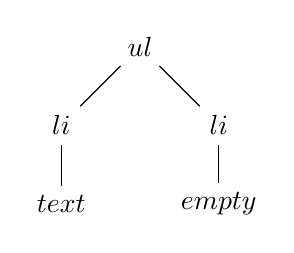
\begin{tikzpicture}[auto]
				\node (and) at (2, 3) {$ul$};
				\node (or1) at (1, 2) {$li$};
				\node (or2) at (3, 2) {$li$};
				\node (true1) at (1, 1) {$text$};
				\node (true2) at (3, 1) {$empty$};

				\draw [-] (and) to (or1);
				\draw [-] (and) to (or2);
				\draw [-] (or1) to (true1);
				\draw [-] (or2) to (true2);
			\end{tikzpicture}
		\end{center}
\end{frame}

\begin{frame}{Determinization}{Now for NFTAs (3)}
	\begin{example}
		\(Q_f = \{q_{ul }\}\)
		\newline
		\(\Delta = \{
					ul(q_{li1},q_{li2}) \rightarrow q_{ul}, ul(q_{li2},q_{li1}) \rightarrow q_{ul}, \newline
					li(q_{text},q_{text}) \rightarrow q_{li1}, li(q_{text}, q_{text}) \rightarrow q_{li2}\newline
					text \rightarrow q_{text}, empty \rightarrow q_{empty}, \newline
					\epsilon(q_{empty}) \rightarrow q_{text}
		\}\)
	\end{example}
	\begin{block}{}
		\begin{itemize}
			\item {
				Use \(\epsilon-closure(q)\) instead of \(q\) for all \(q \in Q\)
			}
			\item {
				Start with the ground terms
			}
			\item {
				Generate target states "on the fly" (=set of possible states in original \(Q\))
			}
			\item {
				Repeat for all states including the newly generated ones
			}
		\end{itemize}
	\end{block}
\end{frame}


\begin{frame}{Determinization}{Now for NFTAs (4)}
	\begin{example}
		\(Q_f = \{q_{ul }\}\)
		\newline
		\(\Delta = \{
					ul(q_{li1},q_{li2}) \rightarrow q_{ul}, ul(q_{li2},q_{li1}) \rightarrow q_{ul}, \newline
					li(q_{text},q_{text}) \rightarrow q_{li1}, li(q_{text}, q_{text}) \rightarrow q_{li2}\newline
					text \rightarrow q_{text}, empty \rightarrow q_{empty}, \newline
					\epsilon(q_{empty}) \rightarrow q_{text}
		\}\)
	\end{example}
	\begin{block}{}
		rules and states:
		\(
			\newline \pause
			text \rightarrow \{q_{text}\} 
			\newline \pause
			empty \rightarrow \{q_{text}, q_{empty}\}
			\newline \pause
			li(\{q_{text}\}, \{q_{text}\}) \rightarrow \{q_{li1}, q_{li2}\}
			\newline \pause
			li(\{q_{text}, q_{empty}\}, \{q_{text}, q_{empty}\}) \rightarrow \{q_{li1}, q_{li2}\}
			\newline \pause
			ul(\{q_{li1}, q_{li2}\}, \{q_{li1}, q_{li2}\}) \rightarrow \{q_{ul}\}
		\)	
	\end{block}
\end{frame}

\begin{frame}{Determinization}{Now for NFTAs (5)}
	\begin{example}
		\begin{itemize}
			\item { 
				\automatonDefinition
			}
			\item {
				\(\Sigma = \{ul, li, text, empty\}\)
			}
			\item {
				\(Q = \{ \{q_{ul}\}, \{q_{text}\},  \{q_{text}, q_{empty}\}, \{q_{li1}, q_{li2}\}\}\}\)
			}
			\item {
				\(Q_f = \{ \{q_{ul}\} \}\)
			}
			\item {
				\(\Delta = \{		text \rightarrow \{q_{text}\},
							\newline
							empty \rightarrow \{q_{text}, q_{empty}\},
							\newline
							li(\{q_{text}\}, \{q_{text}\}) \rightarrow \{q_{li1}, q_{li2}\},		
							\newline
							li(\{q_{text}, q_{empty}\}, \{q_{text}, q_{empty}\}) \rightarrow \{q_{li1}, q_{li2}\},
							\newline
							ul(\{q_{li1}, q_{li2}\}, \{q_{li1}, q_{li2}\}) \rightarrow \{q_{ul}\}
				\}\)
			}
		\end{itemize}
	\end{example}
\end{frame}

\begin{frame}{Determinization}{Now for NFTAs (6)}
	\begin{example}
		\begin{itemize}
			\item { 
				\automatonDefinition
			}
			\item {
				\(\Sigma = \{ul, li, text, empty\}\)
			}
			\item {
				\(Q = \{q_{ul}, q_{text}, q_{text2}, q_{li}\}\)
			}
			\item {
				\(Q_f = \{ q_{ul} \}\)
			}
			\item {
				\(\Delta = \{		text \rightarrow q_{text},
							\newline
							empty \rightarrow q_{text2},
							\newline
							li(q_{text}, q_{text}) \rightarrow q_{li},		
							\newline
							li(q_{text2}, q_{text2}) \rightarrow q_{li},
							\newline
							ul(q_{li}, q_{li}) \rightarrow q_{ul}
				\}\)
			}
		\end{itemize}
	\end{example}
\end{frame}

\begin{frame}{Minimization}{Context (Definition)}
	\begin{definition}
		A Context \textcolor{olive}{C} is a tree with a hole.
	\end{definition}
	\pause
	\begin{center}
		
\begin{tikzpicture}
			\fill[olive] (0,0) -- (1, 0) -- (2, 1) -- (3, 0) -- (4, 0) -- (2, 2) -- (0,0);
		\end{tikzpicture}
	\end{center}
\end{frame}

\begin{frame}{Minimization}{Context Application}
	\begin{definition}
		\(\textcolor{olive}{C}[\textcolor{orange}{t}]\) is a \textcolor{green}{Context application} of \(\textcolor{orange}{t}\) in the context of 	\(\textcolor{olive}{C}\).
	\end{definition}
	\pause
	\begin{center}
		
\begin{tikzpicture}
			\fill[olive] (0,0) -- (1, 0) -- (2, 1) -- (3, 0) -- (4, 0) -- (2, 2) -- (0,0);
			\fill[orange] (1,0) -- (3,0) -- (2, 1) -- (1,0);
		\end{tikzpicture}	
	\end{center}
\end{frame}

\begin{frame}{Minimization: Myhill-Nerode}{Congruence (Definition)}
	\begin{definition}
		A congruence is an equivalence relation on trees closed under context:
		\newline
		\(t_1 \equiv t_2 \Rightarrow \forall C: C[t_1] \equiv C[t_2]\)
	\end{definition}
	\pause
	\begin{center}
		
\begin{tikzpicture}
			\fill[orange] (1,0) -- (3,0) -- (2, 1) -- (1,0);
		\end{tikzpicture}
		\(\equiv\)
		
\begin{tikzpicture}
			\fill[yellow] (1,0) -- (3,0) -- (2, 1) -- (1,0);
		\end{tikzpicture}
	\end{center}
\end{frame}

\begin{frame}{Minimization: Myhill-Nerode}{Congruence (Definition)}
	\begin{definition}
		A congruence is an equivalence relation on trees closed under context:
		\newline
		\(t_1 \equiv t_2 \Rightarrow \forall C: C[t_1] \equiv C[t_2]\)
	\end{definition}
	\begin{center}
		
\begin{tikzpicture}
			\fill[olive] (0,0) -- (1, 0) -- (2, 1) -- (3, 0) -- (4, 0) -- (2, 2) -- (0,0);
			\fill[orange] (1,0) -- (3,0) -- (2, 1) -- (1,0);
		\end{tikzpicture}
		\(\equiv\)
		
\begin{tikzpicture}
			\fill[olive] (0,0) -- (1, 0) -- (2, 1) -- (3, 0) -- (4, 0) -- (2, 2) -- (0,0);
			\fill[yellow] (1,0) -- (3,0) -- (2, 1) -- (1,0);
		\end{tikzpicture}
	\end{center}
	\pause
	\begin{definition}
		For a tree language \(L\) we can define the congruence in \(L\) \(\equiv_L\): \newline
		\(t_1 \equiv_L t_2\) if \(\forall\) Contexts \(C\): \(C[t_1] \in L \iff C[t_2] \in L\)
	\end{definition}
\end{frame}

\begin{frame}{Minimization: Myhill-Nerode}{Definition}
	\begin{theorem}
		The following are equivalent:
		\begin{itemize}
			\item{
				\(L\) is a regular tree language
			}
			\item{
				\(L\) is the union of some congruence classes of finite index
			}
			\item{
				the relation \(\equiv_L\) is a congruence of finite index
			}
		\end{itemize}
	\end{theorem}
	\pause
	\begin{block}{}{}
		\(\Rightarrow sizeof(A_{min}) =\) number of equivalence classes in \(L\)
	\end{block}
\end{frame}

\begin{frame}{Minimization}{Example (1)}
	\begin{example}
		\begin{itemize}
			\item { 
				\automatonDefinition
			}
			\item {
				\(\Sigma = \{ul, li, text, empty\}\)
			}
			\item {
				\(Q = \{q_{ul}, q_{text}, q_{text2}, q_{li}\}\)
			}
			\item {
				\(Q_f = \{ q_{ul} \}\)
			}
			\item {
				\(\Delta = \{		text \rightarrow q_{text},
							\newline
							empty \rightarrow q_{text2},
							\newline
							li(q_{text}, q_{text}) \rightarrow q_{li},		
							\newline
							li(q_{text2}, q_{text2}) \rightarrow q_{li},
							\newline
							ul(q_{li}, q_{li}) \rightarrow q_{ul}
				\}\)
			}
		\end{itemize}
	\end{example}
\end{frame}

\begin{frame}{Minimization}{Example (1)}
	\begin{example}
		\begin{itemize}
			\item { 
				\automatonDefinition
			}
			\item {
				\(\Sigma = \{ul, li, text, empty\}\)
			}
			\item {
				\(Q = \{q_{ul}, \textcolor{red}{q_{text}, q_{text2}}, q_{li}\}\)
			}
			\item {
				\(Q_f = \{ q_{ul} \}\)
			}
			\item {
				\(\Delta = \{		text \rightarrow q_{text},
							\newline
							empty \rightarrow q_{text2},
							\newline
							\textcolor{red} {
								li(q_{text}, q_{text}) \rightarrow q_{li},	
							}	
							\newline
							\textcolor{red} {
								li(q_{text2}, q_{text2}) \rightarrow q_{li},
							}
							\newline
							ul(q_{li}, q_{li}) \rightarrow q_{ul}
				\}\)
			}
		\end{itemize}
	\end{example}
\end{frame}

\begin{frame}{Minimization}{Example (2)}
	\begin{example}
		\(\Delta = \{		text \rightarrow q_{text},
							\newline
							empty \rightarrow q_{text2},
							\newline
							li(q_{text}, q_{text}) \rightarrow q_{li},
							\newline
							li(q_{text2}, q_{text2}) \rightarrow q_{li},
							\newline
							ul(q_{li}, q_{li}) \rightarrow q_{ul}
		\}\)
	\end{example}
	\begin{center}
  		\begin{tabular}{| l |  l | l | l |  l  |}
    			\hline
   			 			&	 \(q_{text}\) 	& 	\(q_{text2}\) 	& 	\(q_{li}\)  	& 	\(q_{ul}\) 	\\ \hline
   			 \(q_{text}\) 	&	-			&	-			&	-		&	-		\\ \hline
   			 \(q_{text2}\) 	&				&	-			&	-		&	-		\\ \hline
			 \(q_{li}\) 		&				&				&	-		&	-		\\ \hline
			 \(q_{ul}\) 		&				&				&			&	-		\\
    			\hline
 		 \end{tabular}
	\end{center}
\end{frame}

\begin{frame}{Minimization}{Example (3)}
	\begin{example}
		\(\Delta = \{		text \rightarrow q_{text},
							\newline
							empty \rightarrow q_{text2},
							\newline
							li(q_{text}, q_{text}) \rightarrow q_{li},
							\newline
							li(q_{text2}, q_{text2}) \rightarrow q_{li},
							\newline
							ul(q_{li}, q_{li}) \rightarrow q_{ul}
		\}\)
	\end{example}
	\begin{center}
  		\begin{tabular}{| l |  l | l | l |  l  |}
    			\hline
   			 			&	 \(q_{text}\) 	& 	\(q_{text2}\) 	& 	\(q_{li}\)  	& 	\(q_{ul}\) 	\\ \hline
   			 \(q_{text}\) 	&	-			&	-			&	-		&	-		\\ \hline
   			 \(q_{text2}\) 	&				&	-			&	-		&	-		\\ \hline
			 \(q_{li}\) 		&				&				&	-		&	-		\\ \hline
			 \(q_{ul}\) 		&	0			&	0			&	0		&	-		\\
    			\hline
 		 \end{tabular}
	\end{center}
\end{frame}

\begin{frame}{Minimization}{Example (4)}
	\begin{example}
		\(\Delta = \{		text \rightarrow q_{text},
							\newline
							empty \rightarrow q_{text2},
							\newline
							li(q_{text}, q_{text}) \rightarrow q_{li},
							\newline
							li(q_{text2}, q_{text2}) \rightarrow q_{li},
							\newline
							ul(q_{li}, q_{li}) \rightarrow q_{ul}
		\}\)
	\end{example}
	\begin{center}
  		\begin{tabular}{| l |  l | l | l |  l  |}
    			\hline
   			 			&	 \(q_{text}\) 	& 	\(q_{text2}\) 	& 	\(q_{li}\)  	& 	\(q_{ul}\) 	\\ \hline
   			 \(q_{text}\) 	&	-			&	-			&	-		&	-		\\ \hline
   			 \(q_{text2}\) 	&				&	-			&	-		&	-		\\ \hline
			 \(q_{li}\) 		&	1			&	1			&	-		&	-		\\ \hline
			 \(q_{ul}\) 		&	0			&	0			&	0		&	-		\\
    			\hline
 		 \end{tabular}
	\end{center}
\end{frame}

\begin{frame}{Minimization}{Example (5)}
	\begin{example}
		\(\Delta = \{		text \rightarrow q_{text},
							\newline
							empty \rightarrow q_{text2},
							\newline
							li(q_{text}, q_{text}) \rightarrow q_{li},
							\newline
							li(q_{text2}, q_{text2}) \rightarrow q_{li},
							\newline
							ul(q_{li}, q_{li}) \rightarrow q_{ul}
		\}\)
	\end{example}
	\begin{center}
  		\begin{tabular}{| l |  l | l | l |  l  |}
    			\hline
   			 			&	 \(q_{text}\) 	& 	\(q_{text2}\) 	& 	\(q_{li}\)  	& 	\(q_{ul}\) 	\\ \hline
   			 \(q_{text}\) 	&	-			&	-			&	-		&	-		\\ \hline
   			 \(q_{text2}\) 	&	\textcolor{red}{(merge)}	&	-		&	-		&	-		\\ \hline
			 \(q_{li}\) 		&	1			&	1			&	-		&	-		\\ \hline
			 \(q_{ul}\) 		&	0			&	0			&	0		&	-		\\
    			\hline
 		 \end{tabular}
	\end{center}
\end{frame}

\begin{frame}{Minimization}{Minimized Example}
	\begin{example}
		\begin{itemize}
			\item { 
				\automatonDefinition
			}
			\item {
				\(\Sigma = \{ul, li, text, empty\}\)
			}
			\item {
				\(Q = \{q_{ul}, q_{text_{new}}, q_{li}\}\)
			}
			\item {
				\(Q_f = \{ q_{ul} \}\)
			}
			\item {
				\(\Delta = \{		text \rightarrow q_{text_{new}},
							\newline
							empty \rightarrow q_{text_{new}},
							\newline
							li(q_{text_{new}}, q_{text_{new}}) \rightarrow q_{li},	
							\newline
							ul(q_{li}, q_{li}) \rightarrow q_{ul}
				\}\)
			}
		\end{itemize}
	\end{example}
\end{frame}

\begin{frame}{Conclusion}{}
	\begin{itemize}
		\item {
			(ranked) NFTA/DTFAs behave similar to NFA/DFAs
		}
		\item {
			(ranked) NFTAs can be determinized
		}
		\item {
			(ranked) DFTAs can be minimized
		}
	\end{itemize}
\end{frame}

\begin{frame}{}{}
	\begin{center}
		Thank you for the attention!
	\end{center}
\end{frame}

% All of the following is optional and typically not needed. 
\appendix
\section<presentation>*{\appendixname}
\subsection<presentation>*{Sources}

\begin{frame}[allowframebreaks]
  \frametitle<presentation>{Sources}
    
  \begin{thebibliography}{10}
    
  \beamertemplatebookbibitems
  % Start with overview books.

  \bibitem{TATA}
	Hubert Comon, et al.
	\newblock {\em Tree Automata Techniques and Applications, 2007}.
 
  \beamertemplatearticlebibitems

  \bibitem{Martens}
	Prof. Dr. Wim Martens et al.
	\newblock Automata and Logic on Trees
	\newblock {\em http://lrb.cs.uni-dortmund.de/\textasciitilde martens/data/esslli07/lecture01.pdf, http://lrb.cs.uni-dortmund.de/\textasciitilde martens/data/esslli07/lecture02.pdf}, 2007

  \bibitem{Regneri, Stefan Thater}
	Michaela Regneri, Stefan Thater
	\newblock Programmierkurs Python II SS 2011 (Determinization of NFAs)
	\newblock {\em http://www.coli.uni-saarland.de/courses/python2-11/folien/PythonII11-05.pdf}, 2011

  \bibitem{Prof. Dr. J. Giesl et al.}
	Prof. Dr. J. Giesl et al.
	\newblock Formale Systeme, Automaten, Prozesse SS 2010 (Minimization of DFAs)
	\newblock {\em http://verify.rwth-aachen.de/fosap10/uebungen/blaetter/Loesung5.pdf}, 2010

  \end{thebibliography}
\end{frame}

\end{document}